\begin{multicols}{2}
\topic{Deadlock-1}
A set of blocked processes each holding a resource and waiting to acquire a resource held by another process in the set.

\begin{figure}[H]
   \centering
   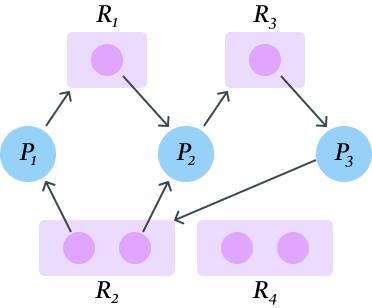
\includegraphics[width=0.5\linewidth]{figures/Deadlock RAG.png}
   \caption*{Resource Allocation Graph with Deadlock}
\end{figure}

\subtopic{Deadlock Characterization}
\begin{itemize}[noitemsep]
    \item \textbf{Mutual exclusion:} only one process at a time can use a resource
    \item \textbf{Hold and wait:} a process holding at least one resource is waiting to acquire additional resources held by other processes
    \item \textbf{No preemption:} a resource can be released only voluntarily by the process holding it, after that process has completed its task
    \item \textbf{Circular wait:} a set of processes $\{P_1, P_2, \ldots, P_n\}$ are waiting for each other in a circular chain.
\end{itemize}

\subtopic{Deadlock Avoidance}
\begin{itemize}[noitemsep]
   \item Simplest and most useful model requires that each process declare the maximum number of resources of each type that it may need.
   \item The deadlock-avoidance algorithm dynamically examines the resource-allocation state to ensure that there can never be a circular-wait condition.
   \item Resource-allocation state is defined by the number of available and allocated resources, and the maximum demands of the processes.
\end{itemize}

% \columnbreak

\subtopic{Deadlock Prevention}
\begin{itemize}[noitemsep]
   \item \textbf{Mutual exclusion:} not required for sharable resources; must hold for non-sharable resources.
   \item \textbf{Hold and wait:} require processes to request and be allocated all resources before execution, or allow processes to request resources only when they have none.
   \item \textbf{No preemption:} if a process holding resources requests a new unavailable resource, all its currently held resources are released and added to the waiting list. The process restarts only when it can reclaim both its old resources as well as the new ones.
   \item \textbf{Circular wait:} impose an ordering of all resource types, and require that each process requests resources in an increasing order of enumeration.
\end{itemize}


\subtopic{Safe State}
\begin{itemize}
    \item When a process requests an available resource, the system must decide if immediate allocation leaves the system in a \textbf{safe state}.

    \item System is in a \textbf{safe state} if there exists a sequence $\langle P_1, P_2, \dots, P_n \rangle$ of all the processes in the system such that for each $P_i$, the resources that $P_i$ can still request can be satisfied by the currently available resources $+$ the resources held by all preceding processes $P_j$, where $j < i$.
    
    \begin{enumerate}
        \item If $P_i$'s resource needs are not immediately available, then $P_i$ can wait until all $P_j$ have finished.
        \item When $P_j$ is finished, $P_i$ can obtain needed resources, execute, return allocated resources, and terminate.
        \item When $P_i$ terminates, $P_{i+1}$ can obtain its needed resources, and so on.
    \end{enumerate}
\end{itemize}


\topic{Deadlock-2}

\subtopic{Banker's Algorithm}
Let, \ $n$ : number of processes \quad $m$ : number of resource types
\begin{itemize}[leftmargin=*]
    \item \textbf{Available}: A vector of length $m$. $Available[j]=k$ $\Rightarrow$ There are $k$ instances of resource type $R_j$ available.

    \item \textbf{Max}: $n \times m$ matrix. $Max[i,j]=k$ $\Rightarrow$ Process $P_i$ may request at most $k$ instances of resource type $R_j$.
    
    \item \textbf{Allocation}: $n \times m$ matrix. $Allocation[i,j]=k$ $\Rightarrow$ Process $P_i$ is currently allocated $k$ instances of resource type $R_j$.
    
    \item \textbf{Need}: $n \times m$ matrix. $Need[i,j]=k$ $\Rightarrow$ Process $P_i$ may need $k$ more instances of resource type $R_j$ to complete its task.
\end{itemize}

 \begin{center}
   $Need[i,j] = Max[i,j] - Allocation[i,j]$

\end{center}

\begin{figure}[H]
   \centering
   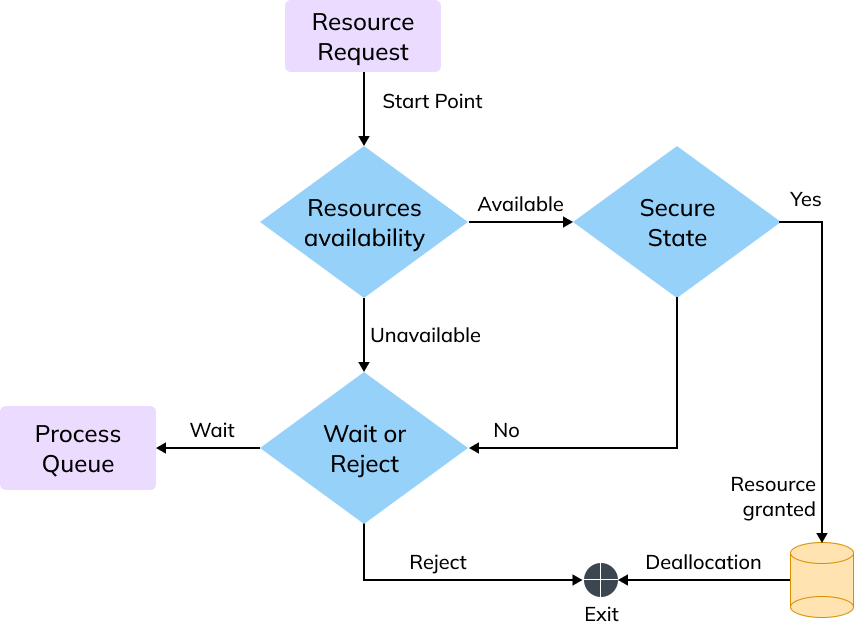
\includegraphics[width=0.9\linewidth]{figures/BankersAlgorithm.png}
\end{figure}   

\columnbreak
\textbf{Safety Algorithm:}
\begin{enumerate}[leftmargin=*, itemsep=0.5em]
   \item Initialization:
   \begin{itemize}
      \item Let \textit{Work} and \textit{Finish} be vectors of length $m$ and $n$, respectively.
      \item $\textit{Work} = \textit{Available}$
      \item $\textit{Finish}[i] = $ false, \quad for $i = 0, 1, \ldots, n-1$
   \end{itemize}
   \item Find an $i$ such that both:
   \begin{enumerate}
      \item \textit{Finish}$[i]$ =  false, and
      \item $\textit{Need}_i \leq \textit{Work}$
   \end{enumerate}
   If no such $i$ exists, go to step 4.
   \item $\textit{Work} = \textit{Work} + \textit{Allocation}_i$ \\
   $\textit{Finish}[i] = $ true; \quad
   Go to step 2.
   \item If $\textit{Finish}[i]$ ==  true for all $i$, then the system is in a safe state.
\end{enumerate}


\subtopic{Resource-Request Algorithm for Process $P_i$}

Let ${Request}_i$ = request vector for process $P_i$. If ${Request}_i[j] = k$, then process $P_i$ wants $k$ instances of resource type $R_j$.

\begin{enumerate}[itemsep=1em]
    \item If ${Request}_i \le {Need}_i$, go to Step 2.
    \par Otherwise, raise an error condition, since process $P_i$ has exceeded its maximum claim.

    \item If ${Request}_i \le {Available}$, go to Step 3.
    \par Otherwise, $P_i$ must wait, since the requested resources are not immediately available.

    \item Pretend to allocate the requested resources to $P_i$ by modifying the state as follows:
    
      ${Available} = {Available} - {Request}_i$ \\
      ${Allocation}_i = {Allocation}_i + {Request}_i$ \\
      ${Need}_i = {Need}_i - {Request}_i$

   \vspace{1em}
   \begin{itemize}[leftmargin=*, noitemsep]
       \item If \emph{safe}, $\Rightarrow$ the resources are allocated to $P_i$.
       \item If \emph{unsafe}, $\Rightarrow$ $P_i$ must wait, and the old resource-allocation state is restored.
   \end{itemize}
\end{enumerate}
\end{multicols}